\documentclass{ximera}

\typeout{Start loading xmPreamble.tex}%

% Add here extra macro's that are loaded automatically by all documents of claas 'ximera' or 'xourse' in this repo

%%
%%  Example:
%%
% \newcommand{\R}{\mathbb{R}

\title{Lesson 2: Making Computations Quickly}
\begin{document}

\begin{abstract}
We continue to explore efficiency in MATLAB.
\end{abstract}

\section*{Lesson 2: Making Many Computations Quickly}

In Lesson 1, we mostly got familiarized with some basic controls and operations in MATLAB, but didn't really do any calculations that would dramatically speed up our work. It wouldn't have taken you too much longer to make the by-hand calculations necessary (or to use a calculator) to solve the problems in Lesson 1.

Now, we're going to slightly increase efficiency, and have MATLAB do many calculations at once. This will still be at a relatively small scale, but we'll begin to do calculations faster than if we had done them by hand. In the next lesson and beyond, we will actually take advantage of MATLAB's capabilities to speed up our work.

\subsection*{Activity 1: Arrays (i.e. lists of numbers)}

First, let's define an array, which for now you can simply think of as an ordered list of objects (usually numbers).

Closed brackets \texttt{[ ]} signify arrays, and you can list any amount of numbers you desire within an array. If you want the array to be horizontal, you separate the numbers by space or by comma. If you want the array to be vertical, you separate the array by semicolon \texttt{";"}.

Let's suppose we have multiple objects' masses and we want to store the masses all at once—we would list them in an array, like below.

\begin{remark}
Note: When working with \texttt{"symbols"}, sometimes you just get long fractions, which aren't that easy to work with. When working with simple numbers, like 2 or \texttt{pi}, or even \texttt{sqrt(2)}, you most consistently get the best result by putting \texttt{sym()} around the most basic part of the number (like 2 or \texttt{pi}).
\end{remark}

\begin{verbatim}
masses = [10 5 20 31 sym(pi)^2 sqrt(sym(2))]
\end{verbatim}

Now use commas to separate some of the numbers to show that it gives the same array.

\begin{verbatim}
% define masses again, but with commas to show it has the same output
\end{verbatim}

Note that because \texttt{sym()} was used for \texttt{pi\^2} and \texttt{sqrt(2)}, the entire array was symbolic. The livescript outputs this array in soft brackets \texttt{( )}. 

If you store an array of decimals (i.e. \texttt{double}) then the array will output with no brackets.

\begin{verbatim}
% define the masses array again, twice.
% first, say masses = double(masses), which converts the masses array to
% decimals and then stores this as the new masses.
% then, rewrite the array without using sym() to see that it yields the same
\end{verbatim}

Now, write the same masses array, but arranged vertically.

\begin{verbatim}
% write "masses_vert" by taking the same numbers in the same order and
% separating them by semicolons ";" within the array.
\end{verbatim}

Note, you can switch an array from vertical to horizontal and vice versa by "transposing", which can be done with a single apostrophe \texttt{'}. 

\begin{verbatim}
% name a variable called masses_2 by transposing masses. The syntax is
% masses'
\end{verbatim}

For most of what we'll be doing, it won't really matter whether arrays are vertical or horizontal, as long as you're consistent. It matters for higher math/physics/engineering, however, so get used to working with both.

\subsection*{Activity 2: Calculations on Arrays}

Now let's use an array to speed up our calculations.

Suppose that the masses defined above have different shapes, each sharing the same volume of 4 (so, they have different densities). We want to know how dense each object is.

Like before, we could separately do the \texttt{density = mass / volume} calculation on each mass, OR we can just divide the entire \texttt{masses} array by the volume.

\begin{remark}
Note: Since \texttt{masses} is defined above, no need to define it again, it's in your workspace.
\end{remark}

\begin{verbatim}
% define a number called "volume" with a value of 4
% define an array called "densities" that divides the "masses" array by the
% "volume" number, using the operation " / ".
\end{verbatim}

Because we're dividing by a single number, MATLAB knows to divide each mass individually by the volume and then make a new array listing all of the densities! This makes our lives much easier in the long run.

Notice that the name \texttt{densities} was descriptive because it was a list of multiple densities. Similarly, \texttt{masses} was defined plurally. Again, it's good to keep your work human interpretable.

Now, suppose that Jenny traveled from home to multiple different locations. She wanted to have each trip take around 30 minutes, so she traveled at different average speeds to reach the locations. The speeds are given below (units m/min).

\begin{verbatim}
speeds = [10; 12; 8/2; 2; 4];
\end{verbatim}

With one calculation, determine how far each location was from her home.

\begin{verbatim}
% make a "time" variable representing the constant time of each trip, then
% multiply that time by the speeds array to get the distances
\end{verbatim}

\subsection*{Activity 3: Commands on Arrays}

Now we'll answer the question: What is the total distance that Jenny traveled making the trips?

We can use a MATLAB command called \texttt{sum()} to add up all of the values of an array. Much like the \texttt{sym()} command earlier, you type out the command word, followed by parenthesis, and include each input for the command in the parenthesis.

\begin{remark}
Note: What I'll call \texttt{"commands"}, other instructors or programmers will call \texttt{"functions"}. This is common in coding, so one might say, “Use the sum function to find the total distance.” I'll say \texttt{"commands"} instead, since we'll be working with mathematical functions as well.
\end{remark}

Remember that the \texttt{distances} variable is already stored in the workspace.

\begin{verbatim}
% name a variable called "total_distance" and calculate its value using the
% sum() command on the "distances" variable.
\end{verbatim}

Notice that the \texttt{sum()} command added up each entry of \texttt{distances} for us and gave us the total.

You should get a total distance of 960 km.

What about the average distance that Jenny traveled?

An average (or "mean") of a data set is one (of a few) ways that we characterize the data by finding a "center" for the data. The mean scales down the total sum of the data by how many data points there are, effectively producing a representative value that balances the data. Visually, you can imagine the data being spread out around this center, much like weights on a scale, where the mean serves as the balance point.

\begin{center}
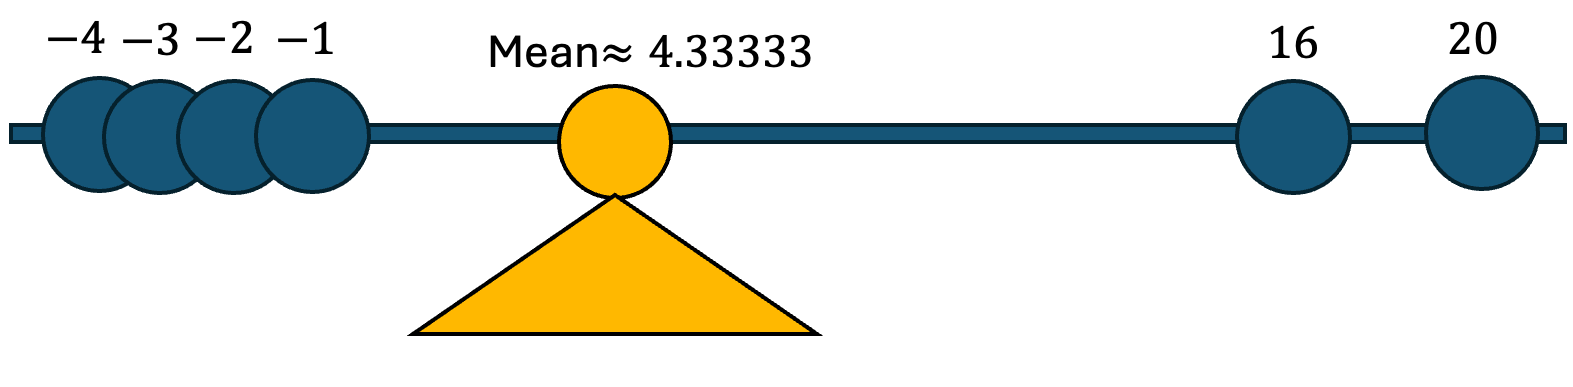
\includegraphics[width=0.6\textwidth]{Mean_Visual.png}
\end{center}

\end{document}